{
\newpage
\newcommand{\scale}{0.65}

\section{Расчёт координат объектов визуального редактора}


Область редактора представляет собой координатную плоскость,
на которой располагаются компоненты бота.
Расположение компонента обеспечивается координатами $ ( x_c , y_c ) $,
которые указывают
на левый верхний угол компонента.

При перемещении компонента вычисляются смещения
$ \bigtriangleup x $ и $\bigtriangleup y$
относительно координат нажатой мыши
$ (x_m, y_m) $ по формулам
\begin{gather}
	\bigtriangleup x = x_c - x_m, \\
	\bigtriangleup y = y_c - y_m.
\end{gather}

Данные смещения используются для расчёта новых координат компонента
$ (x_c', y_c') $ при перемещении мыши с координатами
$ (x_m', y_m') $,
которые вычисляются по формулам
\begin{gather}
	x_c' = x_m' - \bigtriangleup x, \\
	y_c' = y_m' - \bigtriangleup y.
\end{gather}

Расположение компонента на координатной плоскости показано
на рисунке~\ref{f:component-crds}.

\begin{figure}[h]
	\centering
	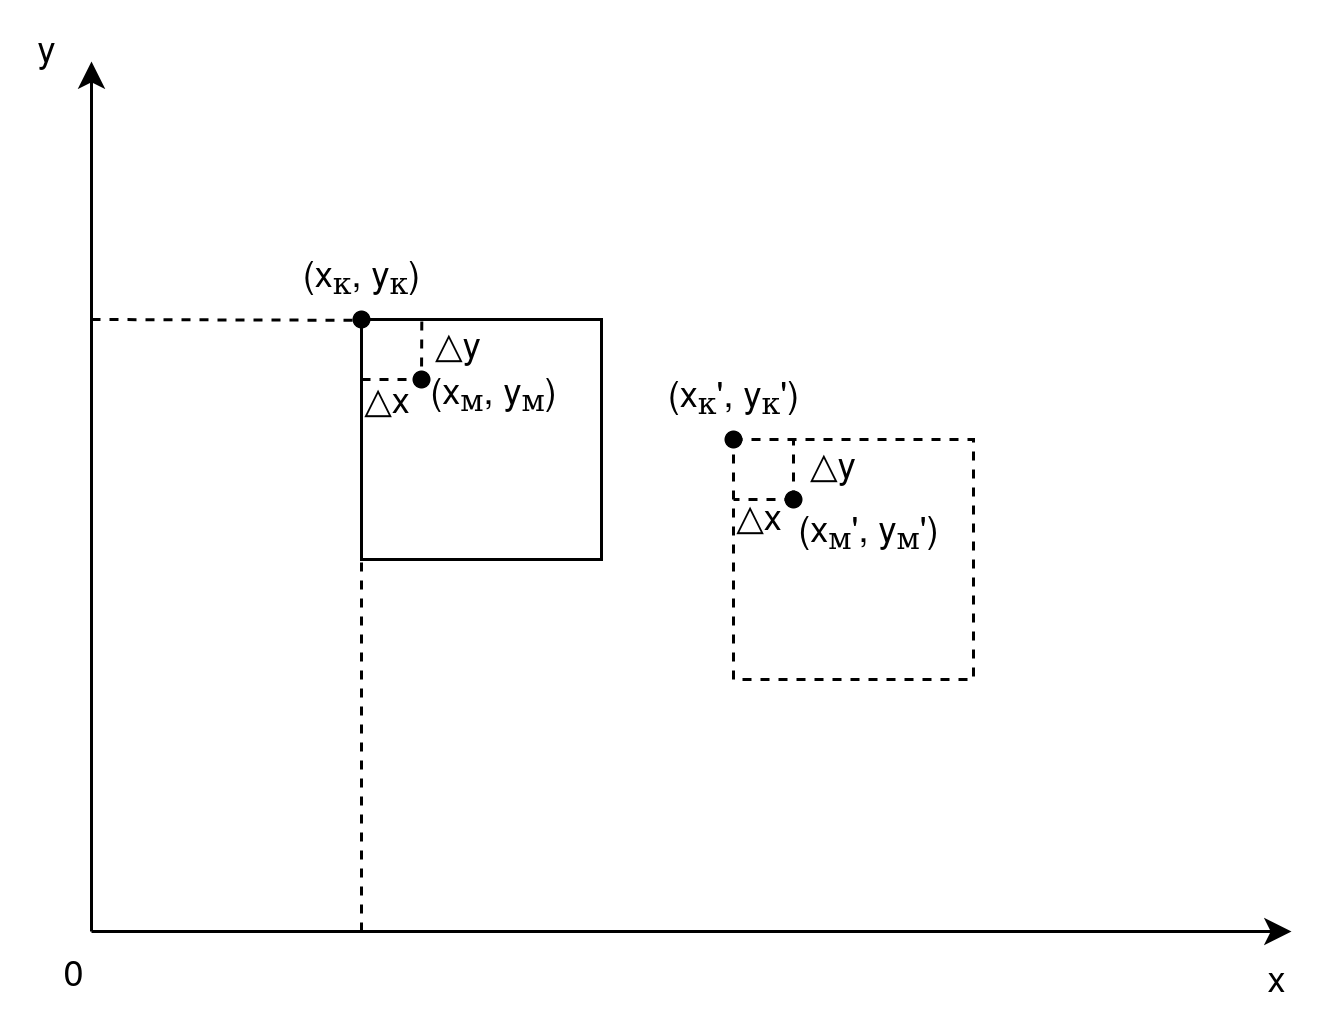
\includegraphics[width=\scale\textwidth]{component-crds}
	\caption{Координаты расположения компонентов}
	\label{f:component-crds}
\end{figure}

Связи между компонентами представляют собой линию со стрелкой.
Линия имеет координаты начала
$ (x_{out}, y_{out}) $
и конца
$ (x_{in}, y_{in}) $, которые представляют собой точки центра окружностей
соединительных точек выхода и входа компонентов.
Расположение связей компонентов на координатной плоскости показано на
рисунке~\ref{f:line-crds}.

\begin{figure}[h]
	\centering
	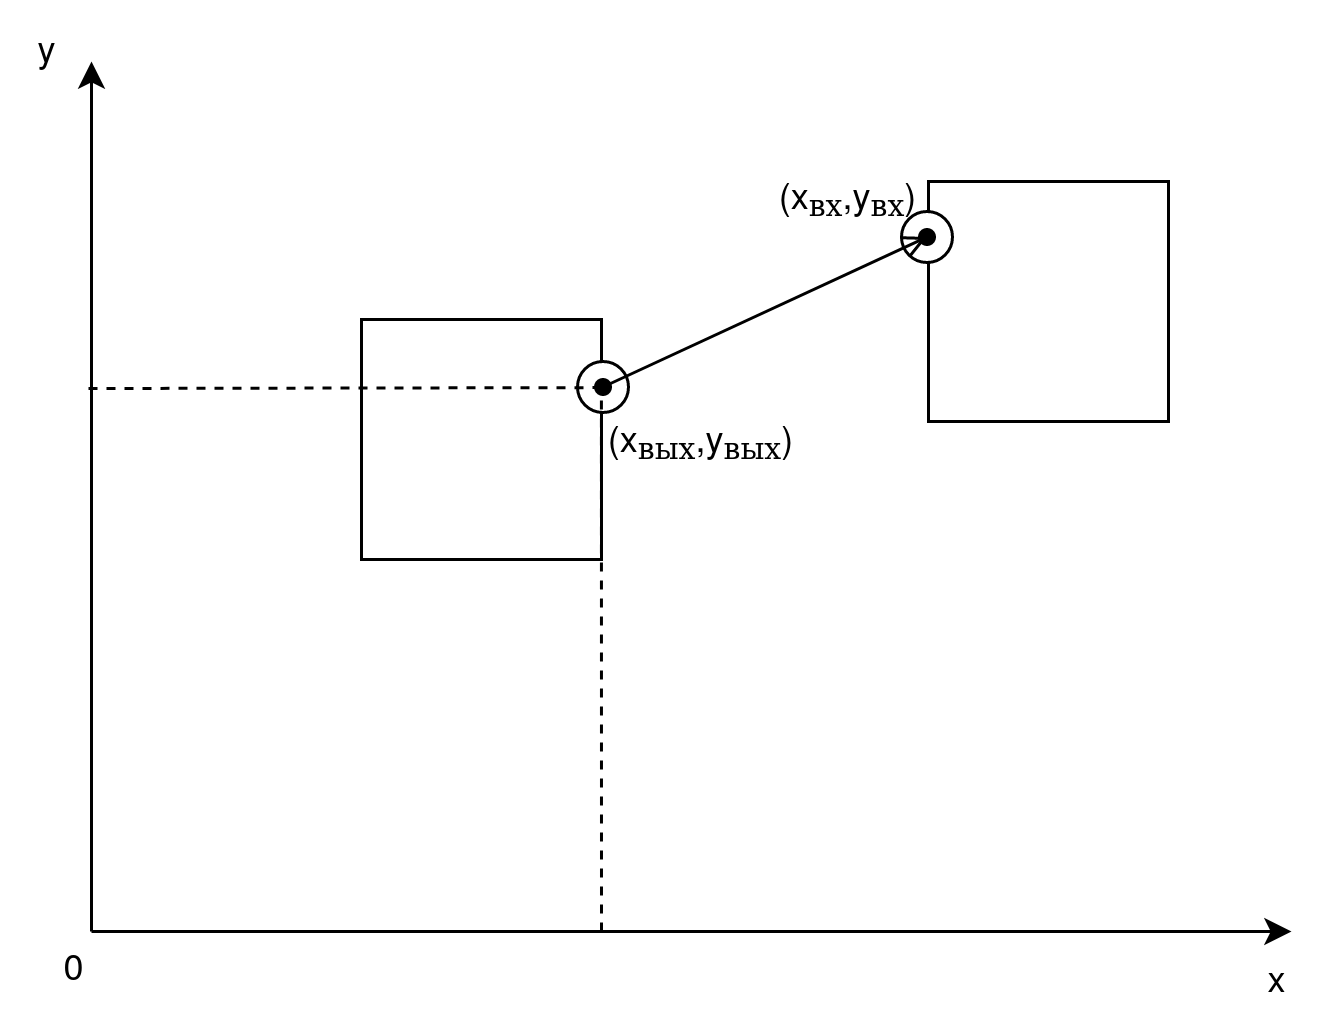
\includegraphics[width=\scale\textwidth]{line-crds}
	\caption{Координаты расположения связей компонентов}
	\label{f:line-crds}
\end{figure}

Стрелка представляет собой две примыкающих к линии прямых.
Стрелка имеет длину
$ a $ и угол между примыкающих прямых $ \alpha $.

Линия между компонентами наклонена под углом $ \beta $ относительно оси $ y $. Угол
вычисляется по формуле
\begin{equation}
	\beta = \arctan(\frac{x_{in} - x_{out}}{y_{in} - y_{out}}).
\end{equation}

Точка
$ (x_a, y_a) $ является окончанием стрелки и её координаты вычисляются по формулам
\begin{gather}
	x_a = x_{in} - sin \beta * a, \\
	y_a = y_{in} - cos \beta * a.
\end{gather}


Расчет смещения $b$ примыкающих прямых относительно основной линии и
смещений $\bigtriangleup x_a$
и $\bigtriangleup y_a$ относительно осей $x$ и $y$ происходит по формулам
\begin{gather}
	b = \tan(\frac{\alpha}{2})*a, \\
	\bigtriangleup x_a = \cos(\beta) * b, \\
	\bigtriangleup y_a = \sin{\beta} * b.
\end{gather}


Сами точки окончания примыкающих прямых
$ (x_{a1}, y_{a1}) $ и $ (x_{a2}, y_{a2}) $
вычисляются по формулам
\begin{gather}
	x_{a1} = x_a + \bigtriangleup x_a, \\
	y_{a1} = y_a - \bigtriangleup y_a, \\
	x_{a2} = x_a - \bigtriangleup x_a, \\
	y_{a2} = y_a + \bigtriangleup y_a.
\end{gather}

Расположение стрелки на координатной плоскости представлено
на рисунке~\ref{f:arrow-crds}.

\begin{figure}[h]
	\centering
	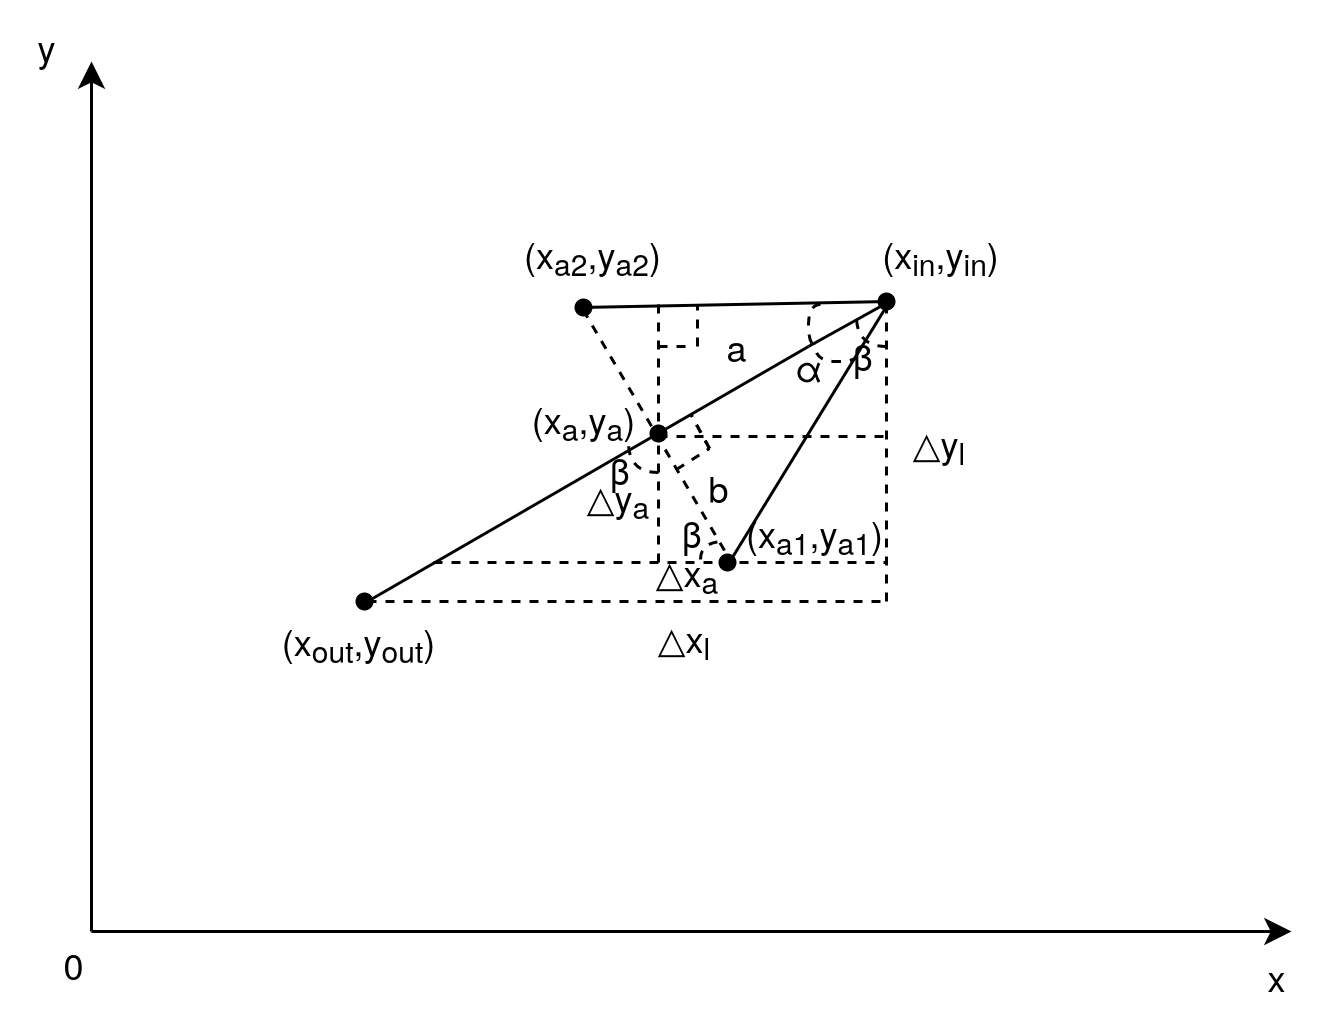
\includegraphics[width=\scale\textwidth]{arrow-crds}
	\caption{Координаты расположения стрелки}
	\label{f:arrow-crds}
\end{figure}


}
